\chapter{Introduction} \label{ch:introduction}

\section{Background}
Approximately 18 million patients are diagnosed with cancer each year \cite{Bray2019}, with reports indicating that up to 50\% of all cases could benefit from radiotherapy (RT) as curative or palliative management of disease (optimal radiotherapy utilisation rate) \cite{Barton2014}. 
Contouring is a critical aspect of RT treatment planning\todo{Is it worth spending one sentence at the beginning here describing what treatment planning itself actually is?}; it describes the process of defining and classifying anatomical regions-of-interest (ROIs) within a patient from medical imaging data \cite{CITATION}.
Contoured regions include: target volumes for treatment, associated error margins; as well as normal tissue regions} (organs at risk - OARs) - for which exposure needs to be minimised to avoid adverse side-effects of treatment \cite{CITATION}. Once ROIs are defined, beam output can be translated to patient anatomy\todo{`beam output can be translated to patient anatomy' reads awkwardly. Maybe, if you define what treatment planning is above, then you can just say here something like, `once the ROIs have been appropriately segmented they can be used within the dose prescription and optimisation stages of treatment planning'}, allowing for dose distributions to be determined for each region (as seen in Figure \ref{fig:contour}). Therefore, contours are part of the primary geometry used to optimise treatment outcomes; achieved by maximising tumour control probability and minimising normal tissue complication probability - i.e. maximising the therapeutic ratio of treatment\todo{The fact that increasing the theraptic ratio is the aim of all this means it likely should be towards the beginng, likely rolled into your treatment planning definition} by optimally distributing dose \cite{CITATION}. As such, accurate contouring is fundamental to the efficacy of RT \cite{CITATION}.

\begin{figure}[!htb]
	\begin{center}
		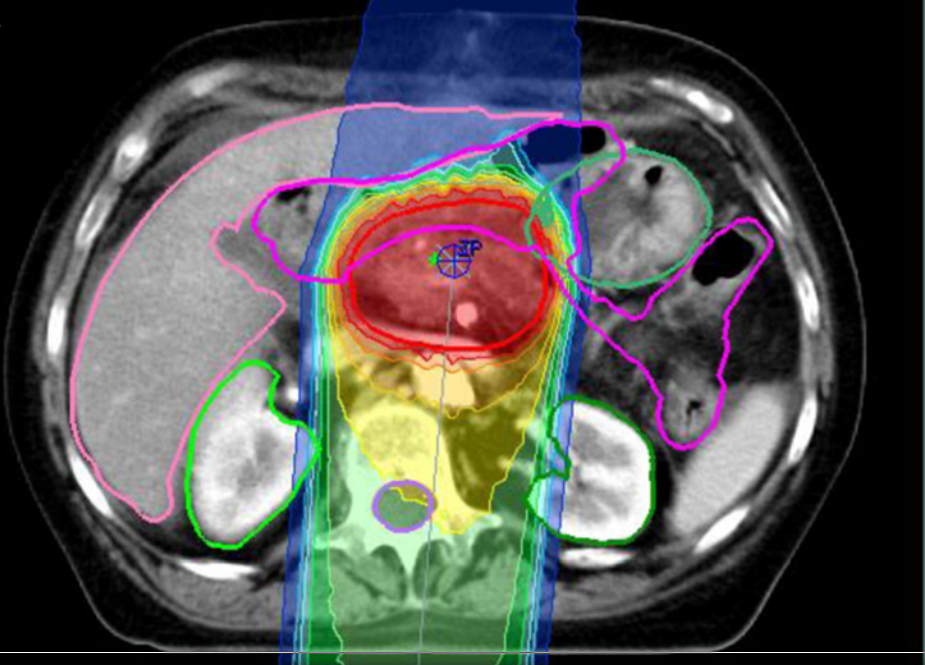
\includegraphics[width=0.5\textwidth]{contour}
		\caption{Single posterior field setup for carbon ion radiotherapy treatment of pancreatic cancer. Multiple contours are outlined on diagnostic CT imaging for treatment planning. Colour map shows the dose distribution over patient anatomy. Figure redrawn from Dreher et al. \cite{Dreher2017}.}
		\label{fig:contour}
	\end{center}
\end{figure}

However, there are current limitations in clinical practice. Large intra- and inter-practitioner (observer) variability (IOV) exists in the definition of ROIs on medical imaging. IOV is a long-standing challenge in RT, and is frequently reported as the largest source of error in accurate treatment delivery \cite{Vinod_2016, tg100}.
Additionally, manual contouring is both time consuming and requires skilled experts \cite{Nikolov_2018}. For instance, research has estimated that a radiation oncologist (RO) needs between 90 -- 120 minutes to delineate pelvic OARs in a cervical cancer patient \cite{Liu_2020}. The process is often computer aided and automatic OAR segmentation tools (i.e. deformable image registration or Atlas-based methods) have both reduced contouring times and improved consistency between expert observers \cite{Vinod_2016}. However, atlas-based methods still require significant manual editing \cite{Nikolov_2018}, and experience difficulty with small organ volumes, regions with poor contrast for differentiation, or high variability in size or location - such as pelvic OARs in prostate and cervical cancer \cite{Schreier_2020, Liu_2020}. Critically, current automatic solutions still present a barrier to the adoption of future technologies that would require fast contouring \cite{Nikolov_2018}. For instance, adaptive radiotherapy has shown the potential to deliver a new standard of care for RT patients by updating treatment plans to daily changes in patient anatomy \cite{Nikolov_2018}. 

In contrast, deep-learning (DL) algorithms have shown significant performance improvements over atlas-methods both in terms of accuracy and time for contour generation \cite{CITATION}. However, the implementation of DL models in clinical environments remains challenging; particularly due to limitations in quantitatively assessing model performance in comparison to expert performance and IOV \cite{Nikolov_2018}. Typical metrics used to quantify the similarity between model and expert contours are volumetric in nature, hence volume overlap tends to be the focus of evaluation \cite{Nikolov_2018}. Recent studies have introduced surface-based performance metrics that aim to provide direct information on the fraction of surface points that require correction to be within IOV tolerances (specific to each OAR) \cite{Nikolov_2018, Vaassen_2020}, and may provide a stronger correlation with time required for contour correction \cite{Vaassen_2020}.

\section{Aim}

U-Net is a type of deep-learning architecture that leverages multi-resolution analysis to perform state-of-the-art segmentation in medical imaging research \cite{Kazemifar_2018, Zhu_2018}\todo{This feels like we're still reading background\ldots}. We present two independent U-Net models in this study, and expand on the original architecture developed by Ronneberger et al. in \cite{Ronneberger_2015}, by integrating recent network\todo{This whole sentence feels like method. I don't believe one should so closely tie ``how it was implemented'' with ``what one sets out to achieve''.}  modifications that have shown improved performance in the literature: 

\textbf{Model 1 - Pelvic imaging QA tool}

Model 1 was designed to fulfil the need for contouring to become part of regular quality assurance due to large IOVs\todo{Actually, it wasn't primarily due to large IOVs, and to be honest here, if it was large IOVs your model shouldn't be designed pick up those issues, because it should let things pass if they are within IOVs. Instead, it is to catch gross contouring errors. An example might be a `left lens' contoured as a `right lens' or whole slices missing from a patient contour.} reported across the literature \cite{Vinod_2016}. In addition, model 1 aims to evaluate the ability of U-Net to achieve expert level performance - as defined by Nikolov et al.'s surface-based performance metric (surface dice similarity coefficient - sDSC) \cite{Nikolov_2018}. We focused on pelvic CT imaging scans, automatically contouring the patient, bladder and rectum volumes\todo{Add a note here about why these were chosen. They were considered to be the most easy organs to auto-contour in this way, chosen with the intent to act as a template for future work extending to other organs.}. The model then compares predicted contours with those created by an expert clinician; and provides feedback on the volumetric overlap (dice similarity coefficient - DSC), as well as the percentage of surface points that deviate by a distance larger than the IOV associated with each structure (sDSC). Recent studies have highlighted that surface overlap metrics - such as the sDSC - may have improved correlation with respect to manual correction times\todo{I believe you've already mentioned this in your lit-review, and if you haven't this should probably be removed from here and put there. -- potentially, remove all references to sDSC, U-Net, etc, and focus just on what the aim was, an aim that could have been fulfilled for example if you had of chosen an atlas method, no matter your method, the project aim didn't change.} required for an automatic segmentation, when compared with standard volumetric overlap metrics \cite{Vaassen_2020}. We present both metrics for comparison, with models trained over a variety of loss functions common to medical image segmentation.

\textbf{Model 2 - Automatic segmentation of vacuum bag structures in canine imaging}

Model 2 was designed to automatically contour vacuum bag structure in canine imaging. Vacuum bag structures are reported to take approximately 30 minutes per patient to contour \cite{CITATION}; hence, this model aims to automate a time-consuming aspect of RT treatment that is typically processed manually in veterinary medicine\todo{Maybe instead: `that is processed manually at the vetinary clinic in question.' It is not standard that vacbags are always contoured. Some clinics may ignore it entirely. Others draw large blobs around the whole thing.}.\todo{This is a much clearer aim}


